\subsection{Chức năng tải file riêng tư (Private file upload)}
\subsubsection{Use case}

\begin{table}[H]
    \centering
    \begin{tabular}{|l|p{11cm}|}
        \hline
        Category & Description \\
        \hline
        Use case name & Private file upload \\
        \hline
        Actor & Sinh viên \\
        \hline
        Assumption & Người dùng đang ở đường dẫn \url{https://school.moodledemo.net/}. Ngôn ngữ của trang web được chỉnh là Tiếng Việt. Người dùng đăng nhập thành công dưới tài khoản sinh viên. Người dùng đang ở trang "Trang chủ".\\\hline
        Normal flow & 
        1. Ở trang chủ, người dùng nhấn chọn vào biểu tượng avatar người dùng. \\
        & 2. Người dùng chọn “Tập tin riêng tư”. \\
        & 3. Hệ thống hiển thị trang tải tập tin.\\
        & 4. Người dùng chọn vào icon “Thêm…” để thêm.\\
        & 5. Người dùng chọn “Choose file”.\\
        & 6. Hệ thống hiển thị cửa sổ chọn file.\\
        & 7. Người dùng chọn file cần tải lên.\\
        & 8. Người dùng chọn “Đăng tải tệp này”.\\
        & 9. Người dùng chọn “Lưu những thay đổi”.\\
        & 10. File được upload thành công.\\\hline
        Alternative flows &
        A1. Tại bước 4:\\
        & 4.1. Người dùng nhấn vào vùng “Thêm các tập tin bằng cách kéo thả”.\\
        & Người dùng tiếp tục thực hiện theo bước 5.\\
        & A2. Tại bước 4:\\
        & 4.1. Người dùng kéo thả file vào vùng “Thêm các tập tin bằng cách kéo thả”.\\
        & Người dùng tiếp tục thực hiện theo bước 9.
        \\\hline
        Exception flows &
        E1. Tại bước 7:\\
        & 7.1 Người dùng chọn file < 1 byte hoặc > 100MB.\\
        & 7.2 Người dùng chọn “Đăng tải tệp này”.\\
        & Hệ thống sẽ báo lỗi kích thước file.\\\hline
    \end{tabular}
    \caption{Use case: Private file upload}
    \label{tab:private-file-upload}
\end{table}

\subsubsection{Activity diagram}
\begin{figure}[H]
    \centering
    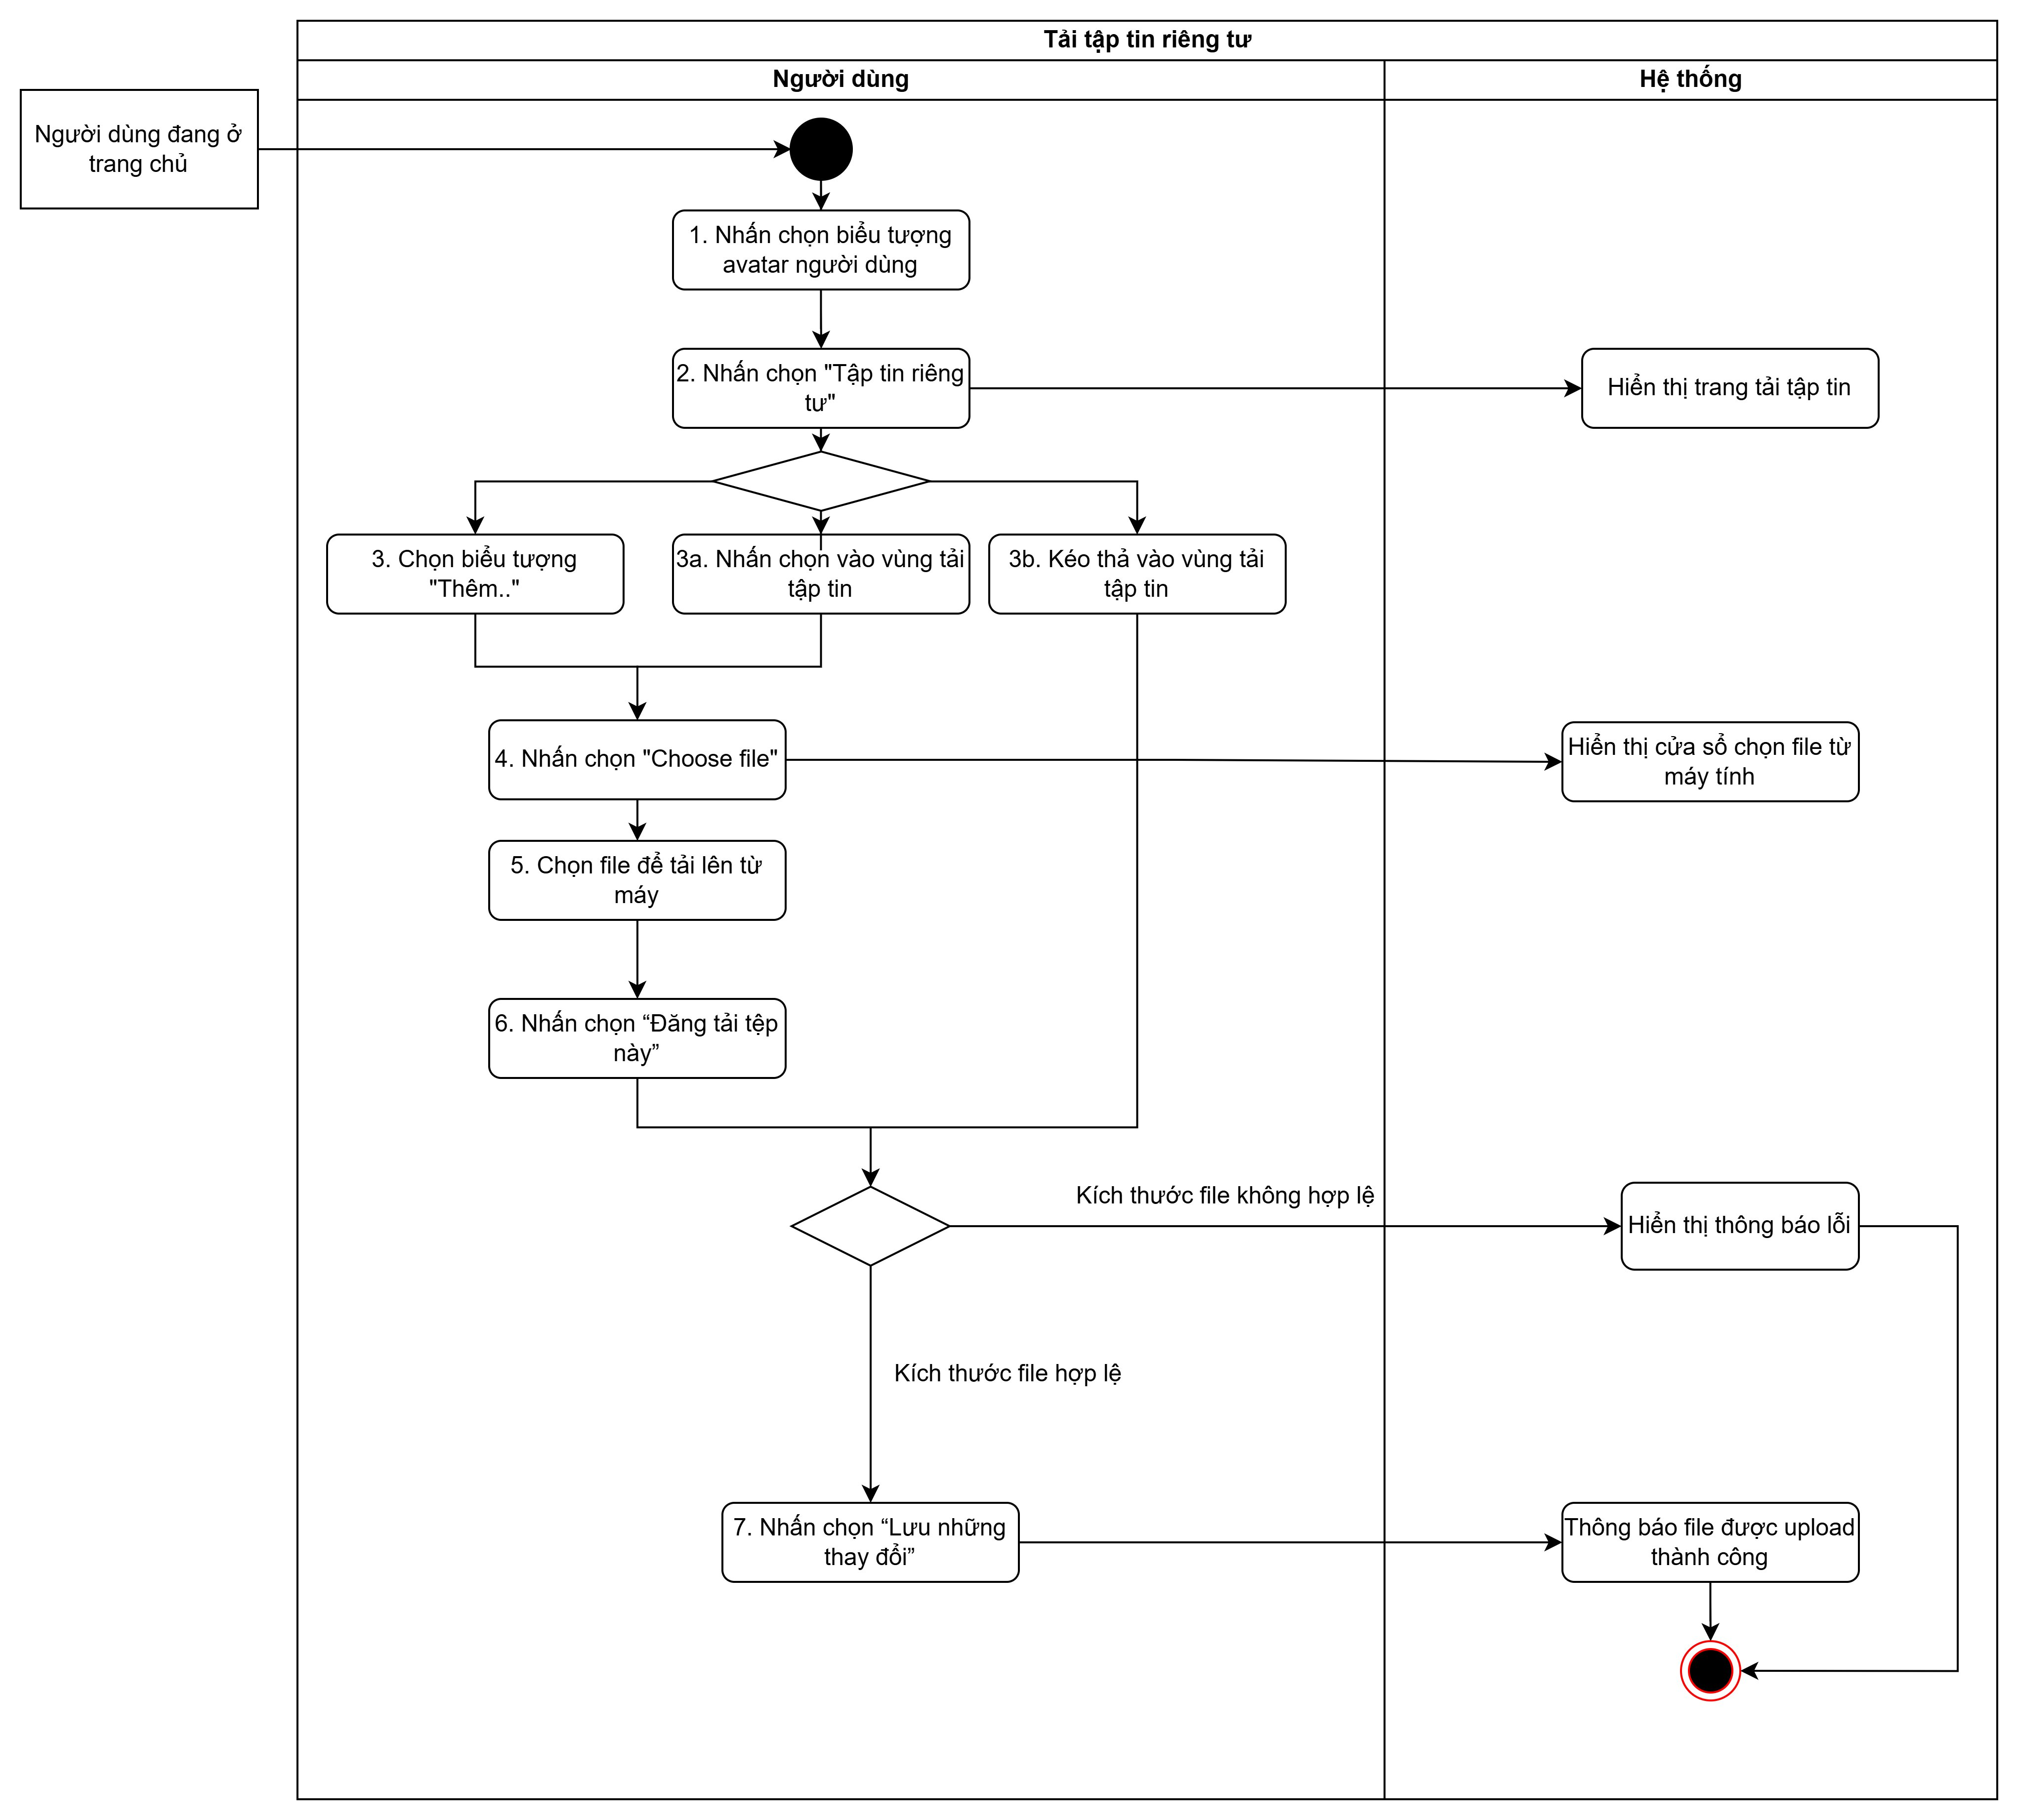
\includegraphics[width=\textwidth]{image/private-file-upload.png}
    \caption{Activity diagram for Private file upload}
    \label{fig:activity-diagram-private-file-upload}
\end{figure}
\subsubsection{Sử dụng phương pháp Boundary value analysis để kiểm thử}
Ta chọn Normal Boundary Value testing, dựa theo các lí do sau:
\begin{itemize}
    \item Kích thước file upload là 1 phạm vi liên tục với biên rõ ràng, lựa chọn BVA phù hợp để kiểm thử các giá trị tại biên, gần biên.
    \item Kiểm tra giá trị biên giúp đảm bảo rằng hệ thống xử lý đúng các tình huống cận biên, nơi dễ phát sinh lỗi nhất.
\end{itemize}
Thay giá trị input ở bước 7 theo domain như sau, gọi x là "Kích thước của file upload" \(1\ \text{byte} \leq x \leq 100\text{MB}\).
\begin{itemize}
    \item PF-001-001: Upload file kích thước giữa 1 byte - 100MB.
    \item PF-001-002: Upload file kích thước nhỏ nhất cho phép.
    \item PF-001-003: Upload file kích thước nhỏ nhất cho phép +.
    \item PF-001-004: Upload file kích thước lớn nhất cho phép -.
    \item PF-001-005: Upload file kích thước lớn nhất cho phép.
\end{itemize}
\subsubsection{Sử dụng phương pháp Equivalence class partitioning}
Lí do chọn: Chức năng upload file dựa trên một phạm vi kích thước liên tục rõ ràng (1 byte - 100 MB). Có thể dễ dàng chia ra lớp tương đương hợp lệ và không hợp lệ. \\
Thực hiện Weak Normal Equivalence Class Testing, chia input ở bước 7 thành các equivalence class như sau:
\begin{itemize}
    \item "Kích thước file" gọi là x, ta chia thành 1 class valid: \(1\ \text{byte} \leq x \leq 100\text{MB}\), 2 class invalid là \(x < 1\ \text{byte}\) và \(x > 100\text{MB}\).
\end{itemize}
Test case:
\begin{itemize}
    \item PF-002-001: Upload file kích thước < 1 byte.
    \item PF-002-002: Upload file kích thước > 100MB
    \item PF-001-001: Upload file kích thước giữa 1 byte - 100MB.
\end{itemize}

\subsubsection{Sử dụng phương pháp Use-case testing để kiểm thử}
Dựa theo Activity diagram, ta chia thành các path:
\begin{itemize}
    \item P1: 1,2,3,4,5,6,7 tương ứng với PF-001-001
    \item P2: 1,2,3a,4,5,6,7 tương ứng với PF-003-001
    \item P3: 1,2,3b,7 tương ứng với PF-003-002
    \item  P4: 1,2,3b tương ứng với PF-003-003
\end{itemize}
\newpage